\section{Processing Unit (Unité de Traitement)}

\subsection{Arithmetic Logic Unit (Unité Arithmétique Logique)}

The Arithmetic Logic Unit (ALU) performs the internal arithmetic manipulation of data 
in the processor. The instructions that are read and executed by the processor control 
the data flow between the registers and the ALU. The instructions also control the 
arithmetic operations performed by the ALU via the ALU’s control inputs. 
A symbolic representation of an ALU is shown in Figure \ref{fig:ALU}.

\begin{figure}[h]
    \centering
    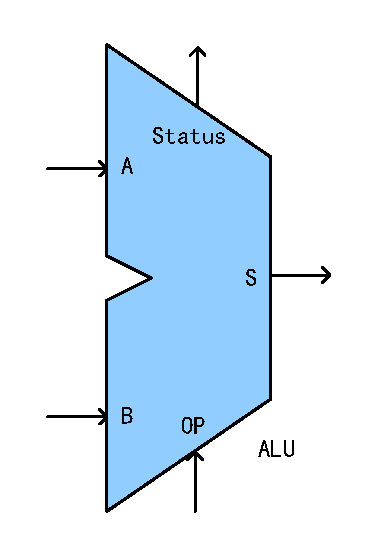
\includegraphics[width=0.3\textwidth]{picture/ALU.pdf}
    \caption{ALU Block Diagram}     
    \label{fig:ALU}
\end{figure}

Where \texttt{A} and \texttt{B} are 32 bits input buses, 
\texttt{S} is a 32 bits output bus, 
\texttt{OP} is a 2 bits command signal, 
and \texttt{Status} is a Output Signal represent NVCZ (we just consider N here, so it is 1 bit).

For the operation of ALU, we can see from Table \ref{tab: Operation Table}.

Thus, we set the inputs and outputs \texttt{ports} of the \texttt{entity} as follow:
\begin{lstlisting}[style=vhdl,columns=fullflexible]
entity ALU is
    port(
        op:in std_logic_vector(1 downto 0);
        a,b: in std_logic_vector(31 downto 0);
        s: out std_logic_vector(31 downto 0);
        n: out std_logic
    );
end entity;
\end{lstlisting}
    
Whenever instructed by the processor, the ALU performs an operation 
(we consider addition and subtraction, and the detailed table will be given below) on one or more values. These values, called operands , 
are typically obtained from two registers, or from one register and a memory location. 
The result of the operation is then placed back into a given destination register 
or memory location. The status outputs indicate any special attributes about the operation, 
such as whether the result was zero, negative, or if an overflow or carry occurred. \cite{catsoulis2005designing} 
\vspace{2cm}
\begin{table}[htbp]
    \centering
    \caption{Operation Table}
    \label{tab: Operation Table}
    \begin{tabular}{@{}ccc@{}}
    \toprule
    \textbf{OP} & \textbf{S} & \textbf{Remark} \\ \midrule
    00              & S=A+B      & ADD             \\
    01              & S=B        & B               \\
    10              & S=A-B      & SUB             \\
    11              & S=A        & A               \\ \bottomrule
    \end{tabular}
\end{table}

Therefore, we build the \texttt{architecture} of ALU in \texttt{\bf{ALU.vhd}}.

\begin{lstlisting}[style=vhdl,columns=fixed]
architecture behav of ALU is
    signal sign: std_logic_vector(31 downto 0);
begin 

    process (a,b,op)
      begin 
        case op is 
            when"00" => sign <=std_logic_vector(signed(a)+signed(b)); 
            when"01" => sign <= b; 
            when"10" => sign <=std_logic_vector(signed(a)-signed(b)); 
            when"11" => sign <= a;
            when others => sign <= a; 
        end case ;
    end process;

    N <= sign(31);
    s <= sign;

end architecture; 
\end{lstlisting}

%%%%%%%%%%%%%%%%%%%%%%%%%%%%%%%%%%%%%%%%%%%%%%%%%%%%%%%%%%%%%%%%%%%%%%%%%%
\subsection{Register File (Banc de Registres)}

\subsubsection{Design Register File}

Registers are temporary storage locations inside the CPU 
that hold data and addresses.

The register file is the component that 
contains all the general purpose registers 
of the microprocessor. A few CPUs also place 
special registers such as the PC and the status 
register in the register file. Other CPUs keep 
them separate.\cite{dumas2005computer}

A symbolic representation of an Register File is shown in Figure \ref{fig:RF}.


Where \texttt{Clk} is a clock Signal; \texttt{Rst} is a asynchrone reset signal which active at high level;
\texttt{WE} is a enable signal of writing datas and \texttt{Rw} is a 4 bits address bus of writing register;
\texttt{W}, \texttt{A} and \texttt{B} are 32 bits data buses; \texttt{Ra} and \texttt{Rb} are 4 bits address buses of reading register.

Thus, the \texttt{ports} of the \texttt{entity} we defined as follow:

\begin{lstlisting}[style=vhdl]
entity Register_File is 
	port (
		clk, rst, WE : in  std_logic ; 
		Ra, Rb, Rw : in std_logic_vector(3 downto 0);
		A, B : out std_logic_vector(31 downto 0);
		W : in std_logic_vector(31 downto 0)
	);
end entity;
\end{lstlisting}

\begin{figure}[h]
    \centering
    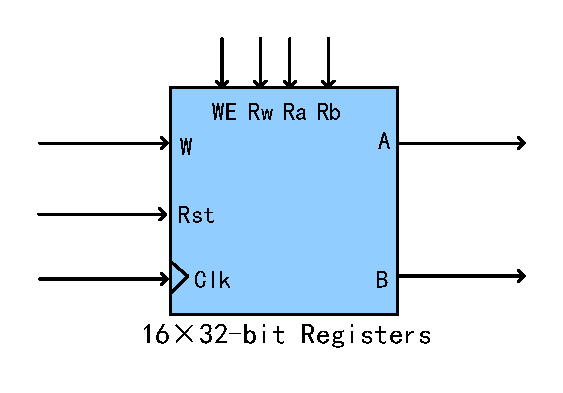
\includegraphics[width = 0.5\textwidth]{picture/16Register.pdf}
    \caption{Register File Block Diagram}     
    \label{fig:RF}
\end{figure}

When \texttt{WE}$ = 1$, which means \textit{enabel to write}, so that we need to write data from bus \texttt{W} to the register on the address \texttt{Rw};
And when \texttt{WE}$= 0$, we will do nothing.
As for reading, it will be done in a combinatorial and simultaneous way.

Therefore, we build the \texttt{architecture} of Register File in \textbf{Registre\_File.vhd}.

\begin{lstlisting}[style=vhdl]
architecture behav of Register_File is
	type matrix is array(15 downto 0) of std_logic_vector(31 downto 0);
	function init_banc return matrix is
		variable result : matrix;
	begin
		for i in 14 downto 0 loop
			result(i) := (others=>'0');
		end loop;
			result(15):=X"00000030";
		return result;
	end init_banc;

	signal Banc: matrix:=init_banc;
begin
	
	A <= Banc(to_integer(unsigned(Ra))); 
	B <= Banc(to_integer(unsigned(Rb))); 

	process(clk, rst) 
	begin 
        if rst ='1' then 
            for i in 14 downto 0 loop
                Banc(i) <= (others=>'0');
            end loop;
                Banc(15)<=X"00000030";
            
        elsif rising_edge(clk) then 
            if WE = '1' then 
                Banc(to_integer(unsigned(Rw)))<=W; 
            end if; 
        end if; 
	end process; 

end architecture;
\end{lstlisting}

\subsubsection{Assemble ALU and Register File}
\label{sec:Assemble ALU and Register File}

We will assemble these two component we have already finished as Figure \ref{fig:AsmbALURF}.

\begin{figure}[htp]
    \centering
    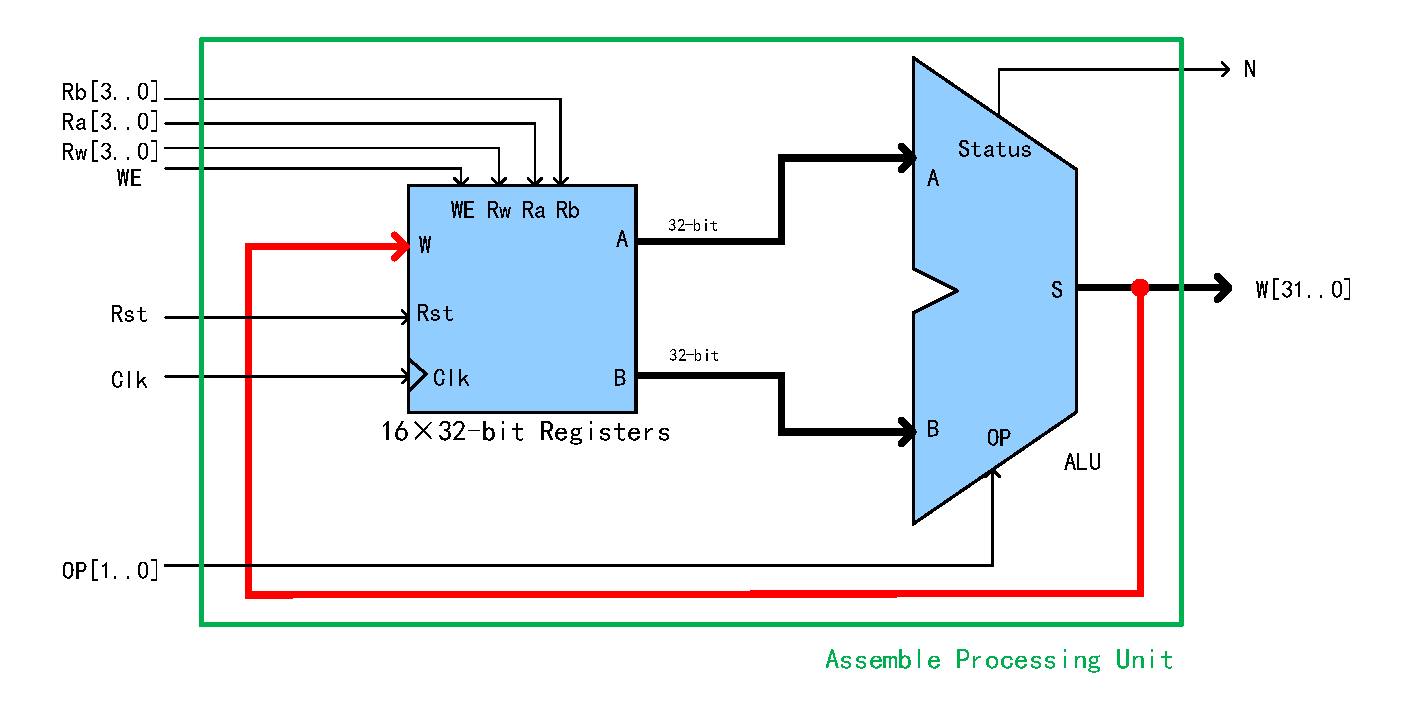
\includegraphics[width = 0.8\textwidth]{picture/AsmbALURF.pdf}
    \caption{Assemble ALU and Register File Block Diagram}     
    \label{fig:AsmbALURF}
\end{figure}

The \texttt{entity} and \texttt{architecture} of \textbf{Assemble\_ALU\_and\_Register\_File.vhd} shows below.

\begin{lstlisting}[style=vhdl, breaklines]
entity Assemble_ALU_and_Register_File is 
    port (
        clk, rst, WE : in  std_logic ; 
        Ra, Rb, Rw : in std_logic_vector(3 downto 0);
        W : out std_logic_vector(31 downto 0);
        N : out std_logic; 
        op : in std_logic_vector(1 downto 0)
    );
end entity;
  
architecture behave of Assemble_ALU_and_Register_File is
    signal busA,busB, busW : std_logic_vector(31 downto 0);
begin
  
    Register_File : entity work.Register_File port map(clk=>clk, rst=>rst, WE=>We, Ra=>Ra, Rb=>Rb, Rw=>Rw, A=>busA, B=>busB, W=>busW); 

    ALU : entity work.ALU port map(a => busA, b=> busB, s => busW, op => op, n => n); 

    W <= busw; 
  
end architecture;
\end{lstlisting}

 And based on the textbench \textbf{Assemble\_ALU\_and\_Register\_File\_tb.vhd} and command file \textbf{Assemble\_ALU\_and\_Register\_File\_test.do}, we test some operations: 
\begin{center}
    \texttt{R(1) = R(15)} \\
    \texttt{R(1) = R(1) + R(15)}\\
    \texttt{R(2) = R(1) + R(15)}\\
    \texttt{R(3) = R(1) – R(15)}\\
    \texttt{R(5) = R(7) – R(15)} 
\end{center}

The simulation result is shown in Figure \ref{fig:AsmbALURFres}. Detailed waves can be found 
as Figure \ref{fig:ModelSim_ assemble_processing_unit_tb(test_bench)} in Appendices \ref{AppendicesA}.

\begin{figure}[htp]
    \centering
    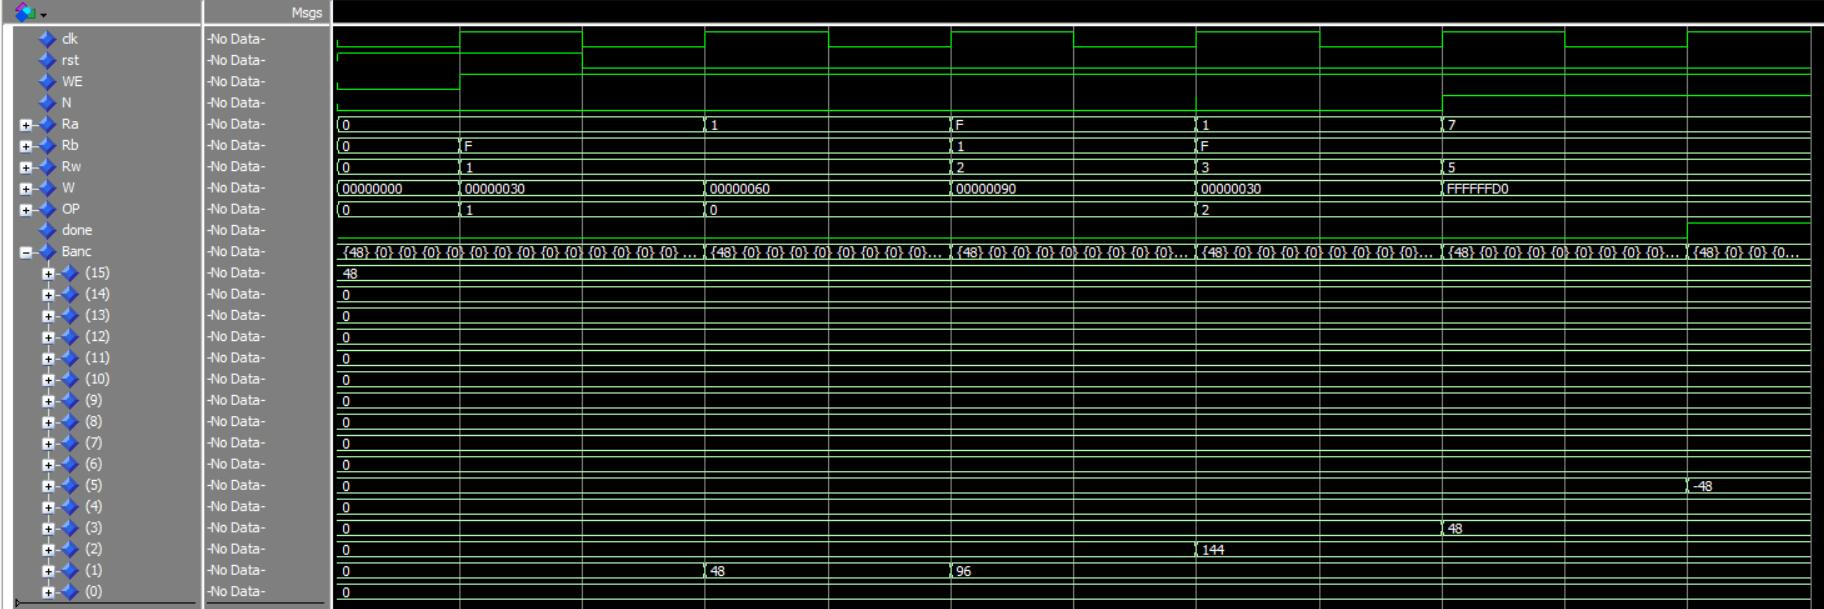
\includegraphics[width=1\textwidth]{picture/AsmbALURFres.jpg}
    \caption{Simulation Waves of Assemble ALU and Regist\_File}     
    \label{fig:AsmbALURFres}
\end{figure}

%%%%%%%%%%%%%%%%%%%%%%%%%%%%%%%%%%%%%%%%%%%%%%%%%%%%%%%%%%

\subsection{2 to 1 Multiplexer (Multiplexeur 2 vers 1)}

This multiplexer has a generic parameter \texttt{N} fixing 
the size of the data input and output. A symbolic representation 
of the multiplexer is shown in Figure \ref{fig:mux21}.

\begin{figure}[htp]
    \centering
    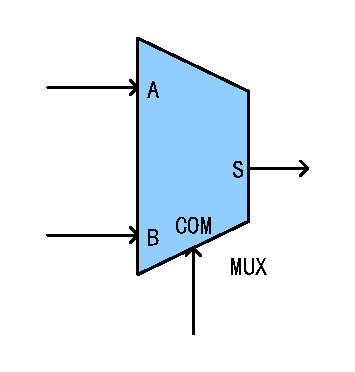
\includegraphics[width=0.3\textwidth]{picture/mux21.pdf}
    \caption{2 to 1 Multiplexer}     
    \label{fig:mux21}
\end{figure}

Where \texttt{A} and \texttt{B} are data inputs, \texttt{S} is data output, and they are all \texttt{N-bit};
\texttt{COM} is a choose signal which is 1 bit. The choose table is as below.

\begin{table}[h]
    \centering
    \caption{MUX Choose Table}
    \label{tab: Choose Table}
    \begin{tabular}{@{}cc@{}}
    \toprule
    \textbf{COM} & \textbf{S} \\ \midrule
    0            & S=A        \\
    1            & S=B        \\ \bottomrule
    \end{tabular}
\end{table}

So we build the component \texttt{MUX} in \textbf{MUX.vhd}.

\vspace{3mm}
\begin{lstlisting}[style=vhdl]
entity MUX is 
    generic (N : positive :=32);

    port (
        S : out std_logic_vector(N-1 downto 0);
        A, B : in std_logic_vector(N-1 downto 0);
        COM : in std_logic
    );
end entity MUX;
  
architecture behave of MUX is
begin
  
    process(A,B,COM)
    begin 
        if COM = '0' then S <= A; 
        elsif COM='1' then S <= B; 
        end if; 
    end process; 
  
end architecture;
\end{lstlisting}

%%%%%%%%%%%%%%%%%%%%%%%%%%%%%%%%%%%%%%%%%%%%%%%%

\subsection{Sign Extension (Extension de Signe)}

This module is used to extend the sign of an input coded 
on \texttt{N bits} to \texttt{32 bits}. It therefore has a generic parameter 
fixing the value of \texttt{N}. A symbolic representation 
of the multiplexer is shown in Figure \ref{fig:SignExtension}.

\begin{figure}[htp]
    \centering
    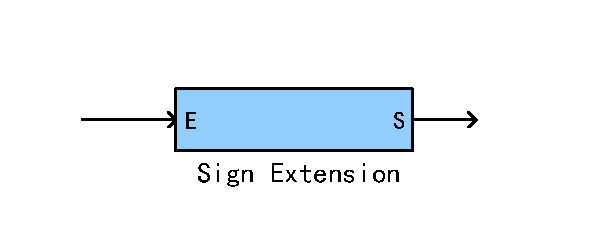
\includegraphics[width=0.5\textwidth]{picture/SignExtension.pdf}
    \caption{Sign Extension Block Diagram}     
    \label{fig:SignExtension}
\end{figure}

Where \texttt{E} is a \texttt{N-bit} data input bus and \texttt{S} is a 32-bit output bus.

And part of its code in \textbf{Sign\_Extension.vhd} shows below.

\begin{lstlisting}[style=vhdl]
entity Sign_Extension is 
    generic (N : positive :=8);
    port (			
        S : out std_logic_vector(31 downto 0);
        E : in std_logic_vector(N-1 downto 0)			
    );
end entity;
  
architecture behav of Sign_Extension is
begin
  
    process(E)
    begin 
        S(N-1 downto 0) <= E; 
        S(31 downto N) <= (others => E(N-1)); 
    end process; 
  
end architecture;
\end{lstlisting}

%%%%%%%%%%%%%%%%%%%%%%%%%%%%%%%%%%%%%%%%%%%%%%%%%%%%%%%%%%

\subsection{Data Memory (Mémoire de Données)}

This memory is used to load and store 64 32-bit words. A symbolic representation 
of the Memory is shown in Figure \ref{fig:DataMem}.

\begin{figure}[htp]
    \centering
    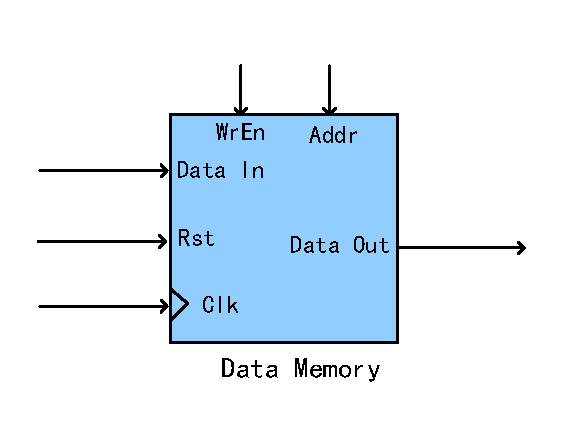
\includegraphics[width=0.5\textwidth]{picture/DataMem.pdf}
    \caption{Data Memory Block Diagram}     
    \label{fig:DataMem}
\end{figure}

Where \texttt{Clk} is a clock Signal; \texttt{Rst} is a asynchrone reset signal which active at high level;
\texttt{WrEn} is a enable signal of writing datas and \texttt{Addr} is a 6 bits address bus;
\texttt{Data In} and \texttt{Data Out} are 32 bits data buses;

Thus, the ports of the entity we defined as follow:

\begin{lstlisting}[style=vhdl]
entity Data_Memory  is 
	port (
		clk, rst, WE : in  std_logic ; 
		Addr : in std_logic_vector(5 downto 0);
		DataOut : out std_logic_vector(31 downto 0);
		DataIn : in std_logic_vector(31 downto 0)
	);
end entity;
\end{lstlisting}

Similar to Register File, when \texttt{WrEn}$=1$, it will write data from \texttt{Data In} to the \texttt{Addr} register;
and when \texttt{WrEn}$=0$, it will do nothing. As for reading, it will be done
in a combinatorial and simultaneous way.

Therefore, we build the \texttt{architecture} of Data Memory in \textbf{Data\_Memory.vhd}

\begin{lstlisting}[style=vhdl]
architecture behave of Data_Memory  is
	type matrix is array(63 downto 0) of std_logic_vector(31 downto 0);
	signal datas: matrix;
begin

	DataOut <= datas(to_integer(unsigned(Addr))); 
	process(clk, rst) 
	begin 
		if rst ='1' then 
			for i in 63 downto 0 loop
				datas(i) <= std_logic_vector(to_unsigned(i,32));
			end loop;
		elsif rising_edge(clk) then 
			if WE = '1' then 
				datas(to_integer(unsigned(Addr)))<=DataIn; 
			end if; 
		end if; 
	end process; 

end architecture;
\end{lstlisting}

%%%%%%%%%%%%%%%%%%%%%%%%%%%%%%%%%%%%%%%%%%%%%%%%%%

\subsection{Assemble Processing Unit (Assemblage Unité de Traitement)}

We assemble all the components we have finished before to make a Processing Unit.
All the signals are readable from the bolck diagram shown as Figure \ref{fig:AsmbUT}.
And we give the part of source code of \textbf{Assemble\_Processing\_Unit.vhd}.

\begin{figure}[htp]
    \centering
    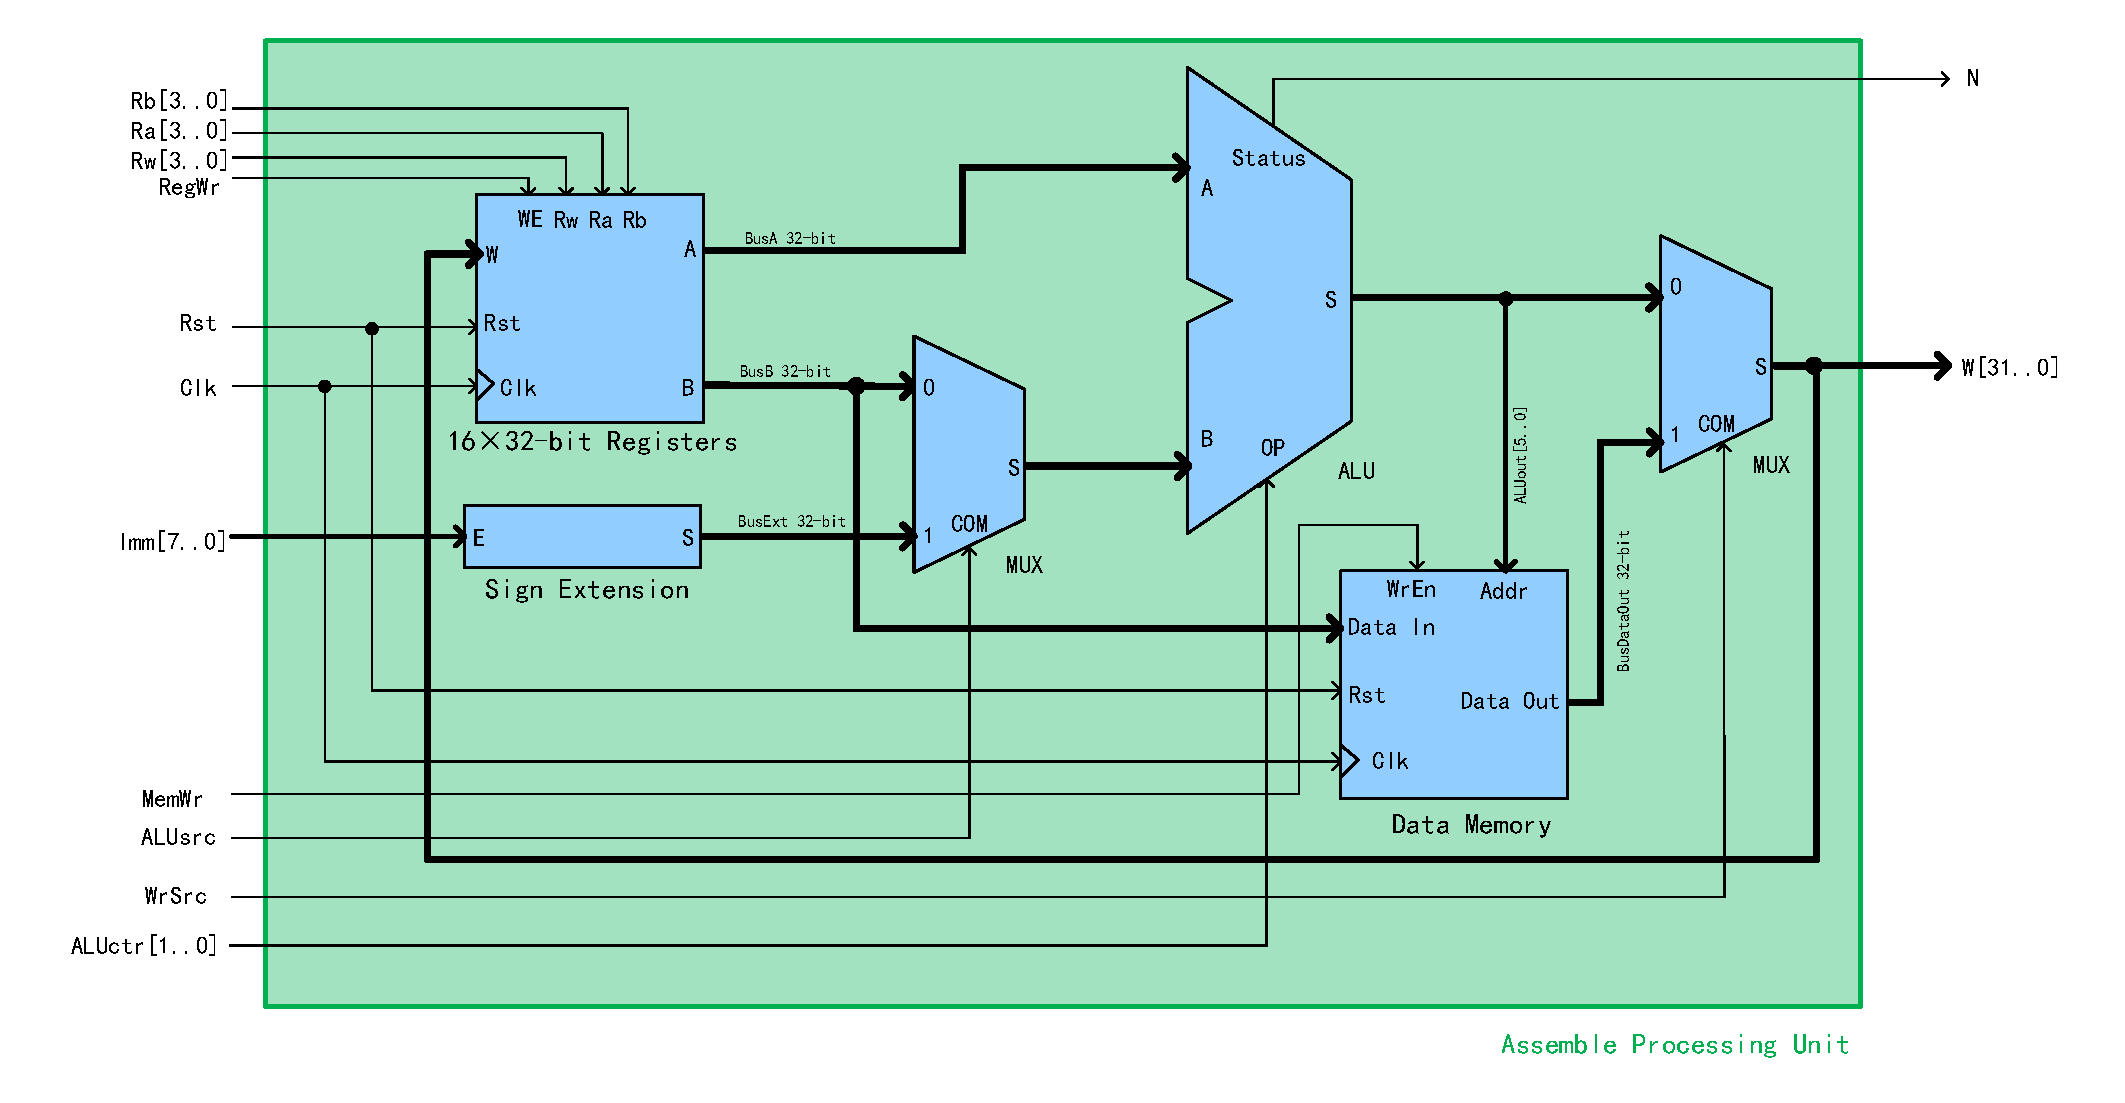
\includegraphics[width=1\textwidth]{picture/AsmbUT.pdf}
    \caption{Assemble Processing Unit Block Diagram}     
    \label{fig:AsmbUT}
\end{figure}

\begin{lstlisting}[style=vhdl, breaklines]
architecture behave of Assemble_Processing_Unit is
    signal busA,busB,ALUS,busExtension,busMux, busW : std_logic_vector(31 downto 0);
    signal DataOut: std_logic_vector(31 downto 0);
begin
  
    Register_File : entity work.Register_File port map(Clk => clk, rst => rst, WE=> RegWr, Ra => Ra, Rb => Rb, Rw => Rw, A => busA, B => busB, W=> busW); 
  
    ALU : entity work.ALU port map(A => busA, B=> busMux, S => ALUS, OP => ALUctr, N => N); 
  
    Sign_Extension : entity work.Sign_Extension port map (E => Imm, S => busExtension);
  
    MUX1 : entity work.MUX port map (A => busB, B=> busExtension, S=> busMux, COM => ALUSrc); 
  
    MUX2 : entity work.MUX port map (A => ALUS, B=> DataOut, S=> busW, COM => WrSrc);
  
    Data_Memory : entity work.Data_Memory port map (Clk => clk, rst => rst, Addr => ALUS(5 downto 0), WE => MemWr, DataIn => busB, DataOut => DataOut); 
    
    W <= busw; 
  
end architecture;
\end{lstlisting}